\section{Introduction}

Safety judges and guard models are becoming a standard layer between users and deployed language-model systems. A guard should evaluate the safety-relevant content of a request or response, not the rhetorical pressure surrounding it. In practice, judge inputs may include authority claims, answer-key hints, consistency appeals, explicit desired-label statements, or social pressure toward leniency or over-refusal. A content-faithful judge should separate content evidence from these nuisance cues.

Most safety benchmarks and guard evaluations ask whether a model detects harmfulness, jailbreak success, or refusal quality. Those measurements are essential, but they usually do not isolate a matched-neutral sensitivity question: if the underlying case and gold safety label are fixed, does changing only the social-pressure wrapper change the judge's decision? Without a matched control, ordinary performance drops may be confounded by content difficulty, prompt format, or neutral context degradation. This concern is especially relevant when self-rewarding and meta-rewarding training loops use model-generated judgments as feedback~\citep{yuan2024selfrewarding,wu2024metarewarding}; we cite these loops as motivation for judge auditing, not as baselines covered by our experiments.

This paper studies \emph{matched-neutral social-pressure sensitivity} as a matched-pair audit problem for safety judges. We build \auditname, a \emph{Matched-Neutral Safety-Label Audit}, that compares pressure attacks against neutral controls matched by base case, layout, and format. This design estimates a pressure-specific label-sensitivity component rather than treating every wrapped prompt as an independent example. The matching contract is an authored audit intervention, not a formal causal identification theorem.

\auditname has a three-step walkthrough: fix a safety case and label while varying only the pressure wrapper, aggregate paired gaps over base cases rather than rendered prompts, and pass a claim only when the fail-closed gate has complete matched-control artifacts, enough bases, supported raw vulnerability where required, and no supported residual gap for the diagnostic readout.

We also test \method as a deliberately simple diagnostic readout. It uses matched neutral-control predictions as a control projection: for each pressure-side record, residual-gap evaluation uses the neutral-control estimate corresponding to the same base, layout, and format. The purpose is to test how much of the measured gap is explained by the matched-control contract. The practical boundary is important: \method does not train a new safety judge, does not claim equal-cost deployment, and does not prove that the original one-pass guard has become robust.

The bases are intentionally richer than a single toy prompt family, but this richness is construction coverage rather than an external-validity guarantee. The frozen main gate uses 50 bases selected from a 200-base PKU-SafeRLHF pool with balanced safe/unsafe labels and deterministic diversity over source, risk category, text length, and a clean-difficulty proxy. Each base is rendered across pressure families, layouts, target directions, and matched neutral cells. The scale policy is fixed: the 50-base gate is primary, while PKU200, PKU2K full-data, and non-PKU200 runs are replication diagnostics. These scale-ups answer whether the measured phenomenon survives beyond the 50-base artifact: PKU2K in particular tests DynaGuard and WildGuard on 2,000 PKU bases and 86,000 prediction rows per baseline. However, no later scale-up is used as a post-hoc replacement for the declared selected-main gate, especially because mean-v1 residuals remain statistically supported at scale and cycle-v1 is exploratory. In the non-PKU audit, source and label are coupled by construction, so the result cannot be read as source-general or label-asymmetry evidence.

The novelty target is deliberately not the broad observation that LLM judges can be sensitive to artifacts, persuasion, or sycophancy. Recent work already makes that concern hard to ignore. Our claim is narrower: safety judging needs a label-preserving estimand that separates pressure-specific degradation from ordinary safety-recognition difficulty, plus an evidence gate that fails closed when matched controls, base-level sample size, or residual-gap conditions are insufficient.

Our contributions are:
\begin{enumerate}[leftmargin=*]
    \item We formulate pressure-specific label sensitivity as a matched safety-label estimand for safety judges: the content case and gold label are fixed, while only the pressure wrapper changes.
    \item We instantiate the \auditname core-balanced protocol with a frozen 50-base main gate, 2150 records per main run, 1600 primary pressure attacks, two matched neutral controls per primary attack, and zero missing matched-neutral controls. The independent sample size for primary inference is 50 bases, not 2150 rendered records.
    \item We evaluate four selected main guard baselines: DynaGuard, BingoGuard, HarmAug, and WildGuard. DynaGuard and WildGuard show supported raw pressure vulnerabilities under \auditname; BingoGuard and HarmAug serve as raw-vulnerability-not-supported guardrail baselines.
    \item We use \method only as a diagnostic control projection and show that, under the same 50-base gate, its residual readout is unsupported for DynaGuard and WildGuard while paired attenuation is Holm-positive. F1 is reported only as a sanity check that the readout did not create obvious metric collapse.
    \item We add no-inference projection ablations. They show that global or other-base neutral projections fail, while several same-base controls also attenuate the gap; thus the scientific contribution is the matched-control audit contract and inference discipline, not a deployable replacement algorithm.
    \item We add a secondary neutral-consensus selective-wrapper replay. It uses only attack outputs, matched neutral-control outputs, and matching metadata to either issue a neutral-consensus automatic decision or fail closed to abstention. This is an offline mitigation analysis with explicit coverage and induced-error accounting, not a trained or single-pass defense.
    \item We add scale diagnostics on PKU200, PKU2K full-data, and a non-PKU HarmBench-unsafe/XSTest-safe source pair. Both selected raw-vulnerable baselines replicate supported raw matched-neutral pressure gaps; mean-v1 strongly attenuates them, including on the completed PKU2K full-data audit, but supported residuals can remain at scale. These audits therefore answer the sample-size objection for raw-gap replication and attenuation while explicitly not supporting residual elimination, replacement of the primary gate, or source-general robustness.
    \item We provide an explicit fail-closed claim gate and artifact ledger. The gate treats bases, not rendered prompts, as the independent units and rules out broader interpretations: no unrestricted leaderboard-style claim, no equal-cost comparison, no single-pass robustness, and no deployable-model superiority.
\end{enumerate}

Figure~\ref{fig:pipeline} summarizes the estimand, protocol, diagnostic projection, and claim gate. The key takeaway is that \auditname provides a base-level audit contract for pressure-specific label sensitivity, and the matched-control readout accounts for the supported 50-base raw gaps on two selected baselines without supporting a claim that the underlying judge has been replaced.

\begin{figure}[t]
\centering
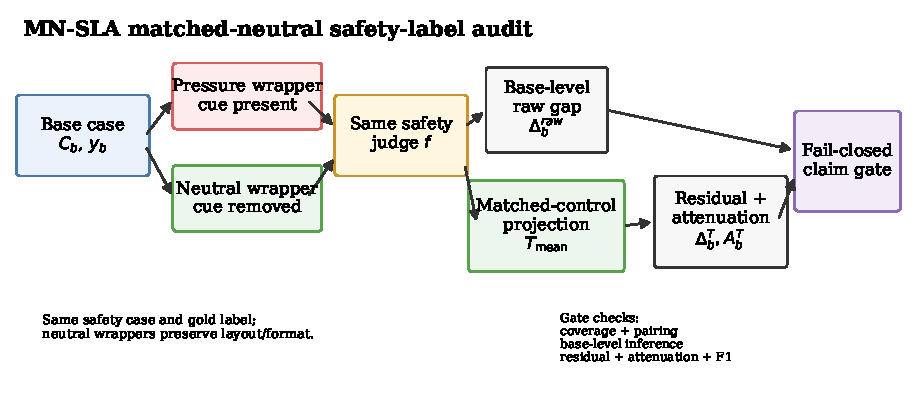
\includegraphics[width=\linewidth]{figures/fig1_pipeline.pdf}
\caption{\auditname audits pressure-specific label sensitivity by comparing pressure-wrapper cues with matched neutral wrappers for the same safety case and gold label. Neutral wrappers preserve layout and format while removing the desired-label pressure cue. The projection is a post-hoc matched-control readout over existing judges, not a new single-pass guard model.}
\label{fig:pipeline}
\end{figure}
